\documentclass{beamer}
\mode<presentation>
\usetheme{CambridgeUS}
\usepackage[russian]{babel}
\usepackage[utf8]{inputenc}
\usepackage[T2A]{fontenc}
\usepackage{sansmathaccent}

\usepackage{verbatim}
\usepackage{alltt}

\pdfmapfile{+sansmathaccent.map}
\title[ER-model]{Модель сущность-связь}
\author{Наумов Д.А., доц. каф. КТ}
\date[01.03.2020] {Базы данных и базы знаний, 2020}

\begin{document}

%ТИТУЛЬНЫЙ СЛАЙД
\begin{frame}
  \titlepage
\end{frame}
  
%СОДЕРЖАНИЕ ЛЕКЦИИ
\begin{frame}
  \frametitle{Содержание лекции}
  \tableofcontents  
\end{frame}
  
%РАЗДЕЛ 1
\section{Проектирование баз данных}
\subsection{Терминология уровней}
\begin{frame}
\begin{block}{Определения}
\begin{itemize}
\item Модель данных — это инструмент описания.
\item Схема базы данных — это результат использования инструмента.
\end{itemize}
\end{block}
\begin{block}{Уровни абстракции данных}
\begin{itemize}
\item Концептуальный уровень соответствует описаниям сущностей (объектов) предметной области, связям между ними. Характерная особенность  полученных  описаний  —  независимость  от используемых моделей данных. 
\item Логический уровень описывает схему базы данных в терминах выбранной модели данных. Скорее всего это будет реляционная модель.
\item Физический уровень соответствует описанию схемы данных в конкретной  СУБД.  Одной  логической  схеме  БД  может соответствовать несколько физических схем для разных СУБД.
\end{itemize}
\end{block}
\end{frame} 

\begin{frame}
\begin{block}{Уровни абстракции данных}
\begin{center}
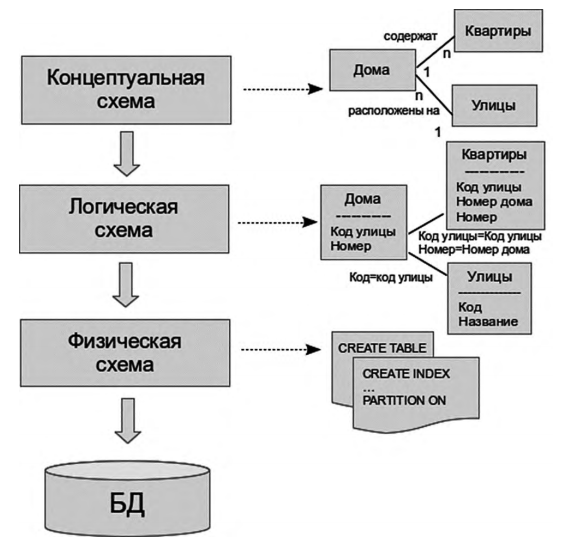
\includegraphics[scale=0.5]{images/levels-01.png}
\end{center}
\end{block}
\end{frame}

\subsection{Концептуальный уровень}
\begin{frame}
\begin{block}{Концептуальный уровень}
\begin{itemize}
\item представляет собой наибольший интерес для функционального специалиста-проектировщика.
\item результат моделирования на концептуальном уровне, который будет использован в логическом проектировании.
\item если концептуальные модели отсутствуют, проектировщику придётся работать «стандартным» методом прочтения линейных текстов многостраничных функциональных спецификаций.
\end{itemize}
\end{block}
\end{frame} 

\subsection{Логический уровень}
\begin{frame}
\begin{block}{Логический уровень}
\begin{itemize}
\item "засилье" реляционных моделй данных.
\item описывая структуры в терминах отношений, ключей, связей, проектировщик может быть уверен, что его результат будет однозначно понят.
\item пgерейдя на сетевую терминологию наборов, записей и агрегатов данных, можно встретить не только непонимание изложенной сути, но и неумение программистов приложений оптимальным
образом работать с данными в выбранной парадигме.
\end{itemize}
\end{block}
\end{frame} 

\subsection{Физический уровень}
\begin{frame}
\begin{block}{Физический уровень}
\begin{itemize}
\item специфика СУБД становится основным фактором эффективности реализации схемы базы данных
вышестоящих уровней.
\end{itemize}
\end{block}
\begin{block}{Соответствие терминов}
\begin{center}
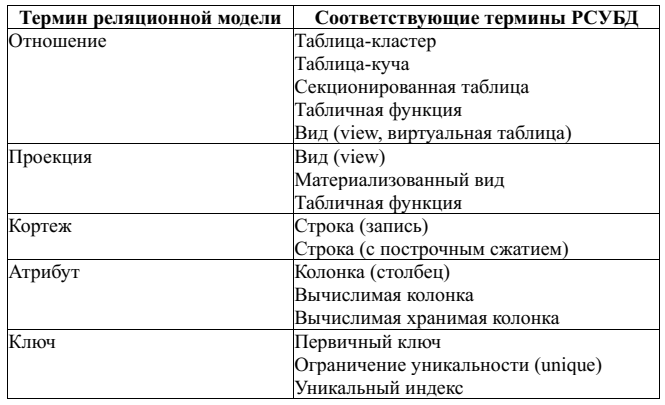
\includegraphics[scale=0.5]{images/rel-dbms.png}
\end{center}
\end{block}
\end{frame} 

\section{Модель Сущность-Связь}
\subsection{Тип сущности}
\begin{frame}
\begin{block}{Тип сущности}
группа объектов в конкретной предметной област с одинаковыми свойствами, имеющая независимое существование.
\end{block}
\begin{center}
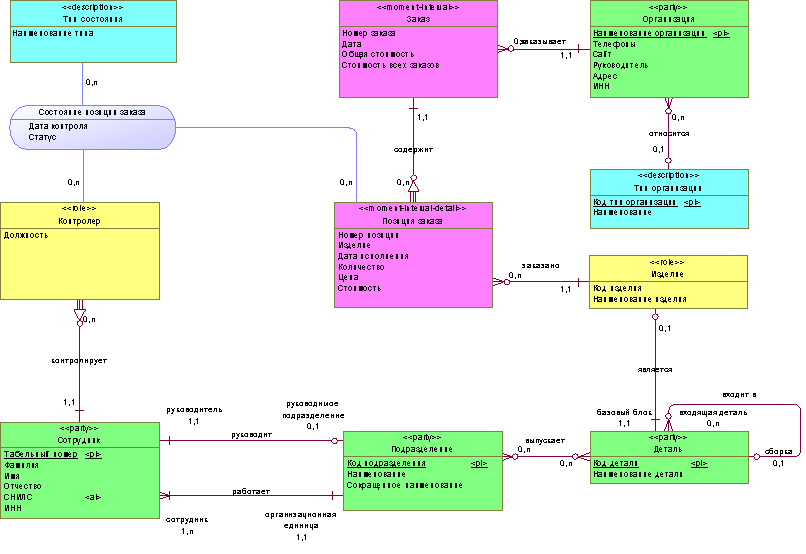
\includegraphics[scale=0.45]{images/shema-er.png}
\end{center}
\end{frame}

\begin{frame}
Тип сущности характеризуется независимым существованием и может быть объектом с физическим  (или реальным) существованием или объектом с концептуальным (или абстрактным)  существованием.
\begin{block}{Физическое существование}
\begin{itemize}
\item Сотрудник
\item Деталь
\item Изделие
\item Организация
\end{itemize}
\end{block}
\begin{block}{Концептуальное существование}
\begin{itemize}
\item Статья затрат
\item Заказ на производство
\end{itemize}
\end{block}
\end{frame}

\begin{frame}
\begin{block}{Экземпляр сущности}
однозначно идентифицируемый объект, который относится к сущности определенного типа.
\end{block}
Каждый тип сущности обозначается именем и характеризуется списком свойств. 
\begin{center}
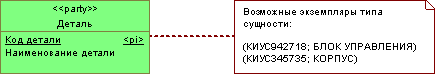
\includegraphics[scale=1.0]{images/entity-type.png}
\end{center}
\end{frame}

\subsection{Тип связи}
\begin{frame}
\begin{block}{Тип связи}
набор осмысленных ассоциаций между сущностями разных типов.
\end{block}
Тип связи (relationship type) является набором ассоциаций между одним (или
несколькими) типами сущностей, участвующими в этой связи. Каждому типу связи присваивается имя, которое должно описывать его назначение. 
\begin{center}
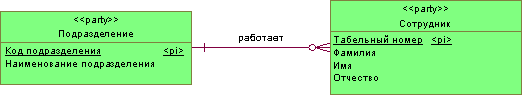
\includegraphics[scale=0.8]{images/relation-01.png}
\end{center}
\end{frame}

\begin{frame}
\begin{block}{Экземпляр связи}
однозначно идентифицируемая ассоциация, которая включает по одному экземпляру сущности из каждого участвующего в связи типа сущности.
\end{block}
Экземпляр связи обозначает все конкретные экземпляры сущности, участвующие в этой связи.
\begin{center}
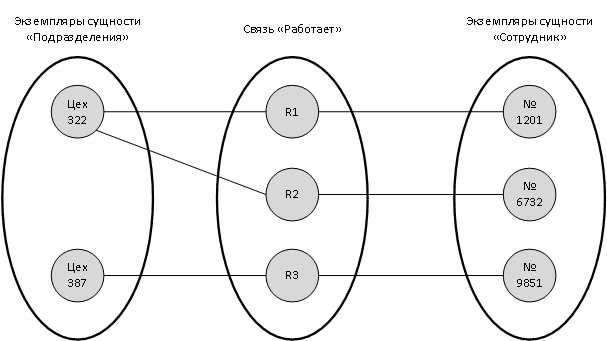
\includegraphics[scale=0.5]{images/relation-02.png}
\end{center}
\end{frame}

\begin{frame}
\begin{block}{Степень типа связи}
количество типов сущностей, которые охвачены данной связью.
\end{block}
\begin{block}{Пример бинарной связи}
\begin{center}
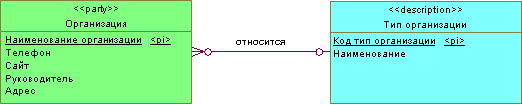
\includegraphics[scale=0.5]{images/relation-03.png}
\end{center}
\end{block}
\begin{block}{Пример тетрарной связи}
\begin{center}
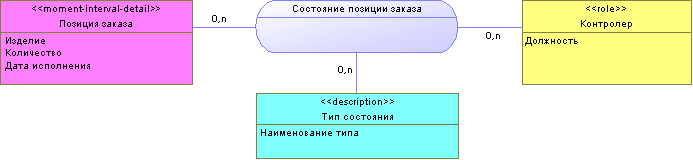
\includegraphics[scale=0.6]{images/relation-04.png}
\end{center}
\end{block}
\end{frame}

\begin{frame}
\begin{block}{Рекурсивная связь}
связь, в которой одни и те же сущности участвуют нескольрко раз в разных ролях.
\end{block}
\begin{block}{Пример рекурсивной связи}
\begin{center}
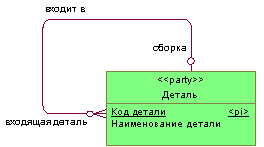
\includegraphics[scale=1.0]{images/self.png}
\end{center}
\end{block}
\end{frame}

\begin{frame}
\begin{block}{Ролевые имена}
Связям могут присваиваться ролевые имена для указания назначения каждой
сущности, участвующей в данной связи. Ролевые имена имеют большое значение в
рекурсивных связях, поскольку позволяют определить функции каждого участника.
\end{block}
\begin{block}{Пример нескольких связей}
\begin{center}
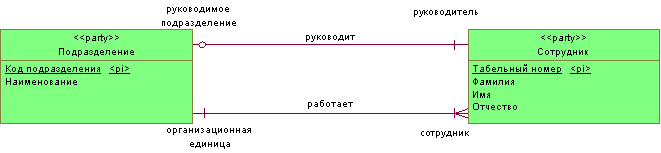
\includegraphics[scale=0.6]{images/role-01.png}
\end{center}
\end{block}
\end{frame}

\subsection{Атрибуты}
\begin{frame}
\begin{block}{Атрибут}
свойство типа сущности или типа связи.
\end{block}
\begin{block}{Домен атрибута}
набор допустимых значений одного или нескольких атрибутов.
\end{block}
\begin{itemize}
\item Простой атрибут - атрибут, состоящий из одного компонента с независимым существованием.
\item Составной атрибут - атрибут, состоящий из нескольких компонентов, каждый из которых характеризуется независимым существованием.
\end{itemize}
\begin{center}
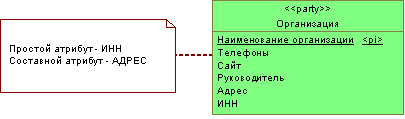
\includegraphics[scale=0.6]{images/simple-attr.png}
\end{center}
\end{frame}

\begin{frame}
\begin{block}{Однозначный атрибут}
атрибут, который содержит одно значение для каждого экземпляра сущности определенного типа.
\end{block}
\begin{block}{Многозначный атрибут}
атрибут, который содержит несколько значений для каждого экземпляра сущности определенного типа.
\end{block}
\begin{center}
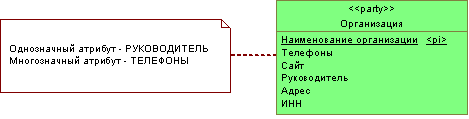
\includegraphics[scale=0.75]{images/many-attr.png}
\end{center}
\end{frame}

\begin{frame}
\begin{block}{Производные (вычисляемые) атрибуты}
атрибут, который представляет значение, производное от значения связанного с ним атрибута или некоторого множества атрибутов, принадлежащих некоторому (не обязательно данному) типу сущности.
\end{block}
Производные атрибуты могут быть связаны:
\begin{itemize}
\item с экземпляром сущности
\item с типом сущности
\item со типом или экземпляром связи
\end{itemize}
\begin{center}
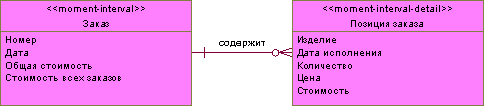
\includegraphics[scale=0.75]{images/attributes.png}
\end{center}
\end{frame}

\subsection{Ключи}
\begin{frame}
\begin{block}{Потенциальный ключ}
атрибут или минимальныйнаборатрибутов, который однозначно идентифицирует каждый экземпляр типа сущности.
\end{block}
\begin{block}{Составной ключ}
потенциальный ключ, который состоит из двух или нескольких атрибутов.
\end{block}
\begin{block}{Первичный ключ}
Потенциальный ключ, который выбран для однозначной идентификации каждого экземпляра сущности определенного типа.
\end{block}
\begin{center}
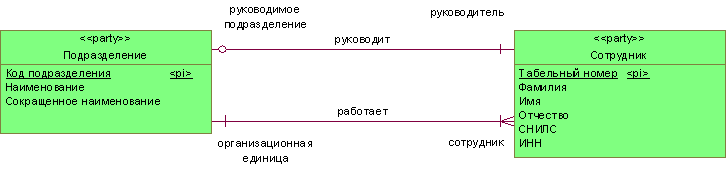
\includegraphics[scale=0.5]{images/keys.png}
\end{center}
\end{frame}

\begin{frame}
\begin{block}{Сущность сильного типа}
тип сущности, существование которого не зависит от какого-то иного типа сущности.
\end{block}
\begin{block}{Сущность слабого типа}
тип сущности, существование которого зависит от какого-то другого типа сущности.
\end{block}
\begin{center}
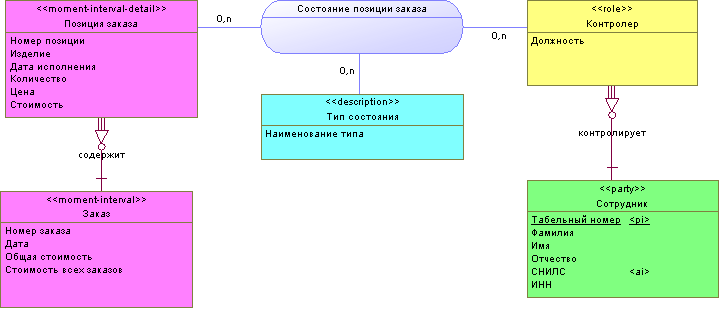
\includegraphics[scale=0.5]{images/depend.png}
\end{center}
\end{frame}

\begin{frame}
\begin{block}{Атрибут связи}
атрибут, который присваивается связи.
\end{block}
\begin{center}
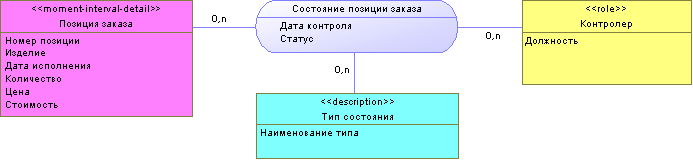
\includegraphics[scale=0.6]{images/rel-attribute.png}
\end{center}
\end{frame}

\subsection{Степень связи}
\begin{frame}
\begin{block}{Степень связи}
условное обозначение количества, возможных экземпляров сущности некоторого типа, которые могут быть связаны с одним экземпляром сущности другого типа с помощью определенной связи.
\end{block}
Виды степеней связей:
\begin{itemize}
\item один-к-одному: 1:1;
\item один-ко-многим: 1:m;
\item многие-ко-многим: m:m;
\end{itemize}
Для определения кратности связи обычно требуется тщательное изучение зависимостей между данными, на которые распространяются ограничения предметной области.
\end{frame}

\begin{frame}
\begin{block}{Cвязь 1:1}
\begin{center}
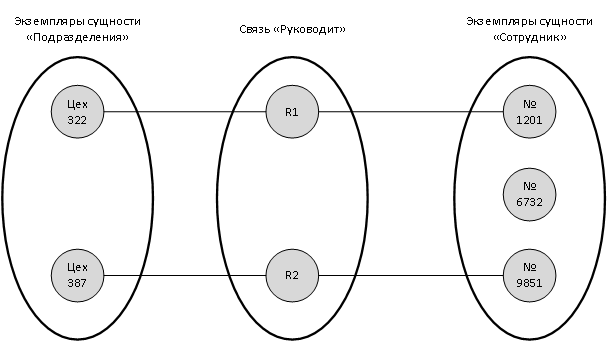
\includegraphics[scale=0.5]{images/one-one.png}
\end{center}
\begin{center}
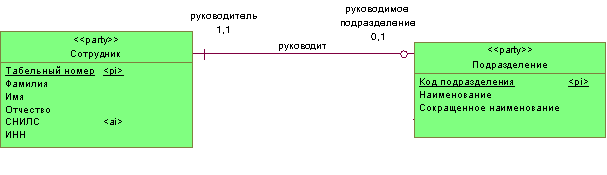
\includegraphics[scale=0.5]{images/one-one-er.png}
\end{center}
\end{block}
\end{frame}

\begin{frame}
\begin{block}{Cвязь 1:m}
\begin{center}
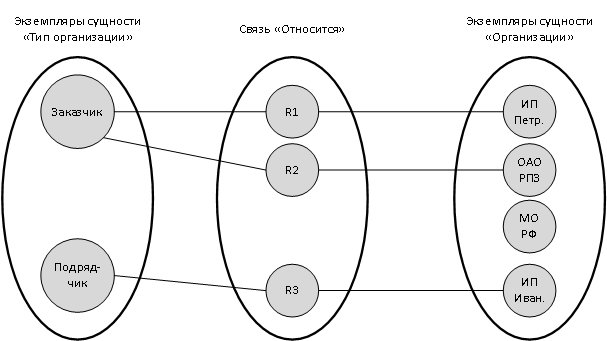
\includegraphics[scale=0.5]{images/one-many.png}
\end{center}
\begin{center}
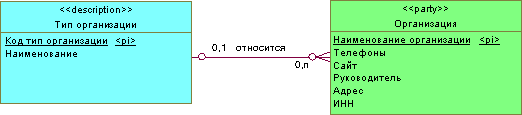
\includegraphics[scale=0.5]{images/one-many-er.png}
\end{center}
\end{block}
\end{frame}

\begin{frame}
\begin{block}{Cвязь m:m}
\begin{center}
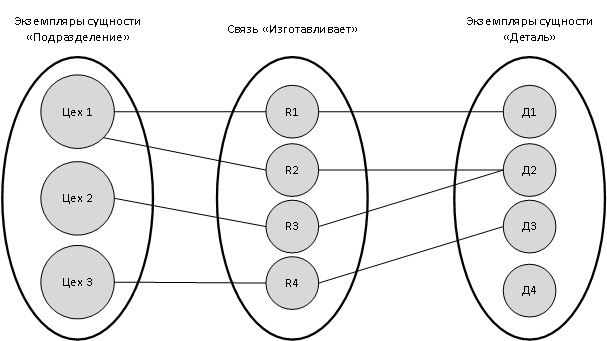
\includegraphics[scale=0.5]{images/many-many.png}
\end{center}
\begin{center}
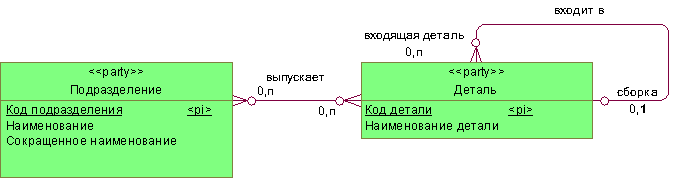
\includegraphics[scale=0.5]{images/many-many-er.png}
\end{center}
\end{block}
\end{frame}

\subsection{Класс принадлежности}
\begin{frame}
\begin{block}{Класс принадлежности}
определяет, участвуют ли в связи все или только некоторые экземпляры сущности.
\end{block}
Виды класса принадлежности:
\begin{itemize}
\item обязательный;
\item необязательный;
\end{itemize}
\begin{center}
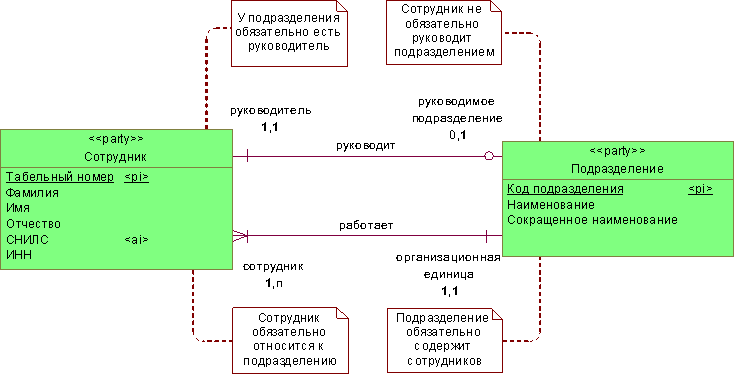
\includegraphics[scale=0.5]{images/requery.png}
\end{center}
\end{frame}

\end{document}